\section{Preliminary Evaluation}
\label{sec:eval}

% \begin{itemize}
%   \item Experiment on datas from the Bureau of Transportation Statistic (\url{http://www.transtats.bts.gov/Fields.asp?Table_ID=236}) to evaluate flight delays by airport
%   \item Infrastructure based on ONE cluster, VM 16.04 LTS (GNU/Linux 4.4.0-53-generic x86\_64), Docker 1.13.0-rc3, Docker Swarm 1.2.5 (discovery: Consul v0.5.2)
%   \item Hardware?
% \end{itemize}
This section presents our preliminary evaluation of \SYS.
First we present our evaluation settings, then the dataset and finally some preliminary benchmark, namely throughput and scalability.

\textbf{Evaluation settings.} We deploy a cluster of virtual machines (VM) based on Ubuntu 16.04 LTS and running a daemon Docker (v.1.13.0-rc3).
Each VM is set with 2 CPU cores and 2GB RAM, and interconnected using a switched 1~Gbps network.
Nodes join a Docker Swarm~\cite{}\vs{FIX} (v1.2.5), and Consul 0.5.2~\cite{}\vs{FIX} as discovery service.
Each VM only execute one single Docker instance, to prevent cross-container interferences\vs{we should add a ref about this}. 
%A single-one container is launch on each node.
Containers leverage the Docker overlay network to comunicate to each other.

\textbf{Dataset.} In our experiments we process a real dataset released by the American Bureau of Transportation Statistic\cite{rita:bts}.
%including each flight's departure and arrivals\cite{statistical_computing:data}.
The dataset reports the flight departures and arrivals of 20 air carriers\cite{statistical_computing:data}.%\ah{pointers on datas are not relevant?}
We implement a simple application on top of \SYS to determine average delays and the total of delayed flights for each air carrier.
%These datas report flights departures and arrivals\cite{rita:bts} and are available on the Statistical Computing\cite{statistical_computing:data}.
We design and implement a simple processing pipeline, that (i) parses the input datasets (in a comma-separated-value format) to data structure (map), (ii) filters by relevancy (i.e. if the data concerns a delayed flight), and (iii) finally reduces to compute to obtain the required informations.\footnote{This experiment is inspired by Kevin Webber's blog entry \emph{Diving into Akka Streams}: \url{https://blog.redelastic.com/diving-into-akka-streams-2770b3aeabb0}.}
We use the 4 last years of the available dataset (from 2005 to 2008), for a total of 28 millions of entries to process and a total size of 2.73 GB.

\textbf{Benchmark: throughput}
This benchmark shows the upload throughtput observed across all cluster while streaming the dataset as fast as possible from the source nodes into the processing pipeline.
We gather banwdwidth measurements by exploting Docker's own monitoring and statistical modules.
%Throughput accross containers wrapping each node of the processing pipeline are measured from Docker stats.
The statistics are gathered at runtime while the experiment is executing.
%During the experiment, we retrieve all the data stats for each container.
%In particular, \texttt{txbytes} stats are extracted to measure containers output throughput.
We present our results in Figure~\ref{fig:throughput}.
In this scenario, only one input source injects the input data into the processing pipeline.
We use a representation based on stacked percentiles. 
The white bar at the bottom represents the minimum value, the pale grey on top the maximal value. 
Intermediate shades of grey represent the 25th, 50th–the median–, and 75th percentiles. 
For instance, the median throughput at 50 seconds into the experiment is at 1500 kB/s, meaning that 50\% of the nodes output data at 1500 kB/s or less.
%These datas are computed to be plotted together by percentile, as shown on figure \ref{fig:throughput}.\ah{maybe it could be relevant to put three plots, corresponding to experiments 4-datas-1-worker, 4-datas-2-workers and 4-datas-4-workers}
With the current implementation, we obseve a peak of 10MB/s upload throughput the processing stages.\vs{for the future, it'd be interesting to know which stage is the fastest one}
%\ah{I gonna measure throuput between two containers run on a swarm cluster, using iperf, for comparison purpose}


\begin{figure}[t!]
  \centering
  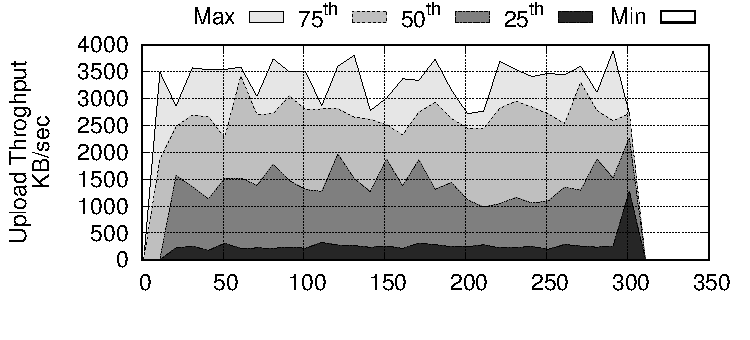
\includegraphics[scale=0.7]{images/tput_upload}
  \caption{Upload Throughput. The middleware completes the processing of the dataset in 305\vs{CHECK} seconds, with a peak of 10 MB/s and an overall throughput of 8.9 MB/s}
  \label{fig:throughput}
\end{figure}

\textbf{Benchmark: scalability}
We also include preliminary scalability results of the \SYS framework.
In particular, we scale up each stage of the processing pipeline, with 1, 2 or 4 workers.
Results are represented on figure \ref{fig:scalability}. 
We present average and standard deviation of the overall completion time of the job, by executing the experiment 20 times for each configuration.
%Scalability of \SYS is evaluated by processing these datas 20 times on 3 different pipeline topology: using 1, 2 or 4 workers for each step of the pipeline.
We observe that by doubling the number of workers from the initial configuration half in two the overall processing time, from 20 minutes to less than 10 minutes.
Convesely, we do not observe these improvements when using 4 workers.
%Results are represented on figure \ref{fig:scalability}, and show clearly better performances between the experiment using only one worker by task, and the one using 2 workers.
%In an other hand, using 4 workers instead of 2 does not show any performance improvement.

\begin{figure}[t!]
  \centering
  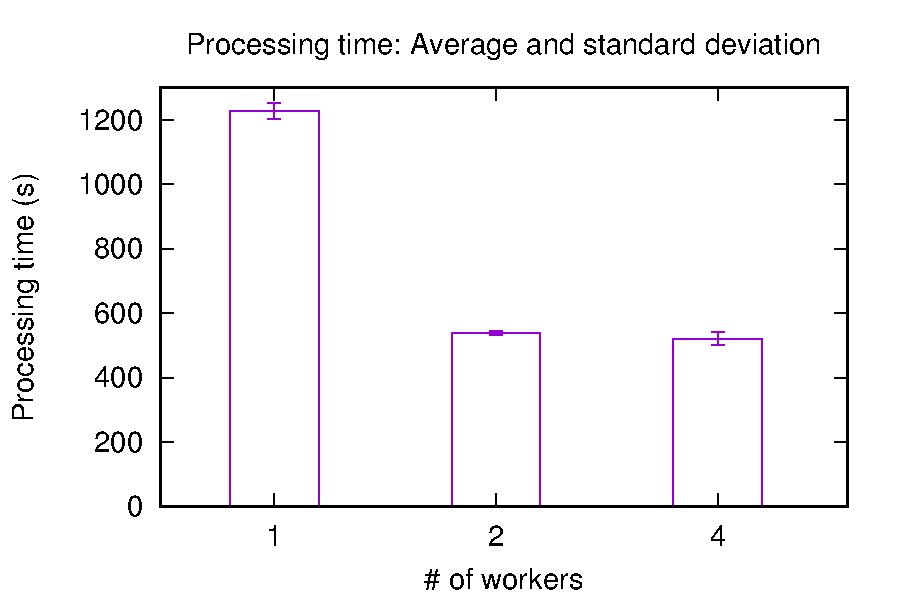
\includegraphics[scale=0.5]{images/avg_stdev_4_streams}
  \caption{Scalability.}
  \label{fig:scalability}
\end{figure}

The latter observation can be explained by the fact that each job in our experiment is very simple and executed too quickly by the workers, compared to the throughput capacity of the communication between two steps of the process pipeline.
This may be due to the limitation of the network bandwith capacity, when the cost of data communication accross nodes is higher than the one of data computation, as described by the Gunther's Universal Law of Computational Scalability\cite{gunther1993simple}, where the relative capacity of a computational platform is inversely proportional to the sum of the levels of contention (e.g., queueing for shared resources) and coherency delay (i.e., latency for data to become consistent) in the system.
In an other hand, it may also be due to the limitation of the router bandwith, the improvement of which is a part of our future work.
